%-------------------------------------------------------------------------------
% Constrói a capa com base na seção de identificação do main.tex
%-------------------------------------------------------------------------------
\begin{capa}
    \setlength{\belowcaptionskip}{0pt}
    \setlength{\abovecaptionskip}{0pt}
    \setlength{\intextsep}{-18pt}
        \begin{figure}[h]
        \begin{center}
            
\includegraphics[scale=1.0]{img/LOGO_UNIVASF_big.pdf}
        \end{center}
      \end{figure}

        %
\includegraphics[scale=0.6]{img/univasf.jpg}
        \center
      {\ABNTEXchapterfont\large\imprimirinstituicao}

      \vspace*{2cm}
          {\imprimirautor}
      \vspace*{2cm}
        \begin{center}
        \ABNTEXchapterfont\bfseries\large\imprimirtitulo
        \end{center}
      \vfill

      \ABNTEXchapterfont\bfseries\large\imprimirlocal\\
      \the\year

      \vspace*{1cm}
\end{capa}
%-------------------------------------------------------------------------------
% Constrói a folha de rosto com base na seção de identificação do main.tex
%-------------------------------------------------------------------------------
\begin{folhaderosto}
    \center
      {\ABNTEXchapterfont\large\imprimirinstituicao}

    \vspace*{2cm}
          {\imprimirautor}
      \vspace*{2cm}
    \vspace*{\fill}

    {\ABNTEXchapterfont\bfseries\large\imprimirtitulo}
    \vspace*{\fill}

    {\hspace{.45\textwidth}
    \begin{minipage}{.5\textwidth}
      \SingleSpacing
      \imprimirpreambulo \\ \\

      {\imprimirorientadorRotulo~\imprimirorientador\par}
      {\imprimircoorientadorRotulo~\imprimircoorientador\par}

    \end{minipage}%
    \vspace*{\fill}}%
    \vspace*{\fill}
      \ABNTEXchapterfont\bfseries\large\imprimirlocal\\
      \the\year
    \vspace*{1cm}
\end{folhaderosto}

%-------------------------------------------------------------------------------
% Constrói a ficha catalográfia com base na seção de identificação do main.tex
% Está comentado porque no final das contas a biblioteca do seu campus que gera a
% numeração, você pode adicionar os numeros aqui, ou anexar o pdf gerado por eles
% ao documento.
%-------------------------------------------------------------------------------
%\begin{fichacatalografica}
%	\vspace*{\fill}					% Posição vertical
%	\hrule							% Linha horizontal
%	\begin{center}					% Minipage Centralizado
%	\begin{minipage}[c]{12.5cm}		% Largura
%
%	\imprimirautor
%
%	\hspace{0.5cm} \imprimirtitulo  / \imprimirautor. --
%	\imprimirlocal, \the\year-
%
%	\hspace{0.5cm} xx p. : il. (algumas color.) ; 30 cm.\\
%
%	\hspace{0.5cm} \imprimirorientadorRotulo~\imprimirorientador\\
%
%	\hspace{0.5cm}
%	\parbox[t]{\textwidth}{\imprimirtipotrabalho~--~\imprimirinstituicao,
%	\the\year.}\\
%
%	\hspace{0.5cm}
%		1. Palavra-chave1.
%		2. Palavra-chave2.
%		I. Orientador.
%		II. Universidade xxx.
%		III. Faculdade de xxx.
%		IV. Título\\
%
%	\hspace{8.75cm} CDU 02:141:005.7\\
%
%	\end{minipage}
%	\end{center}
%	\hrule
%\end{fichacatalografica}

%--------------------------------------------------------------------------------
% Anexando a ficha catalogáfica e a folha de aprovação
%--------------------------------------------------------------------------------
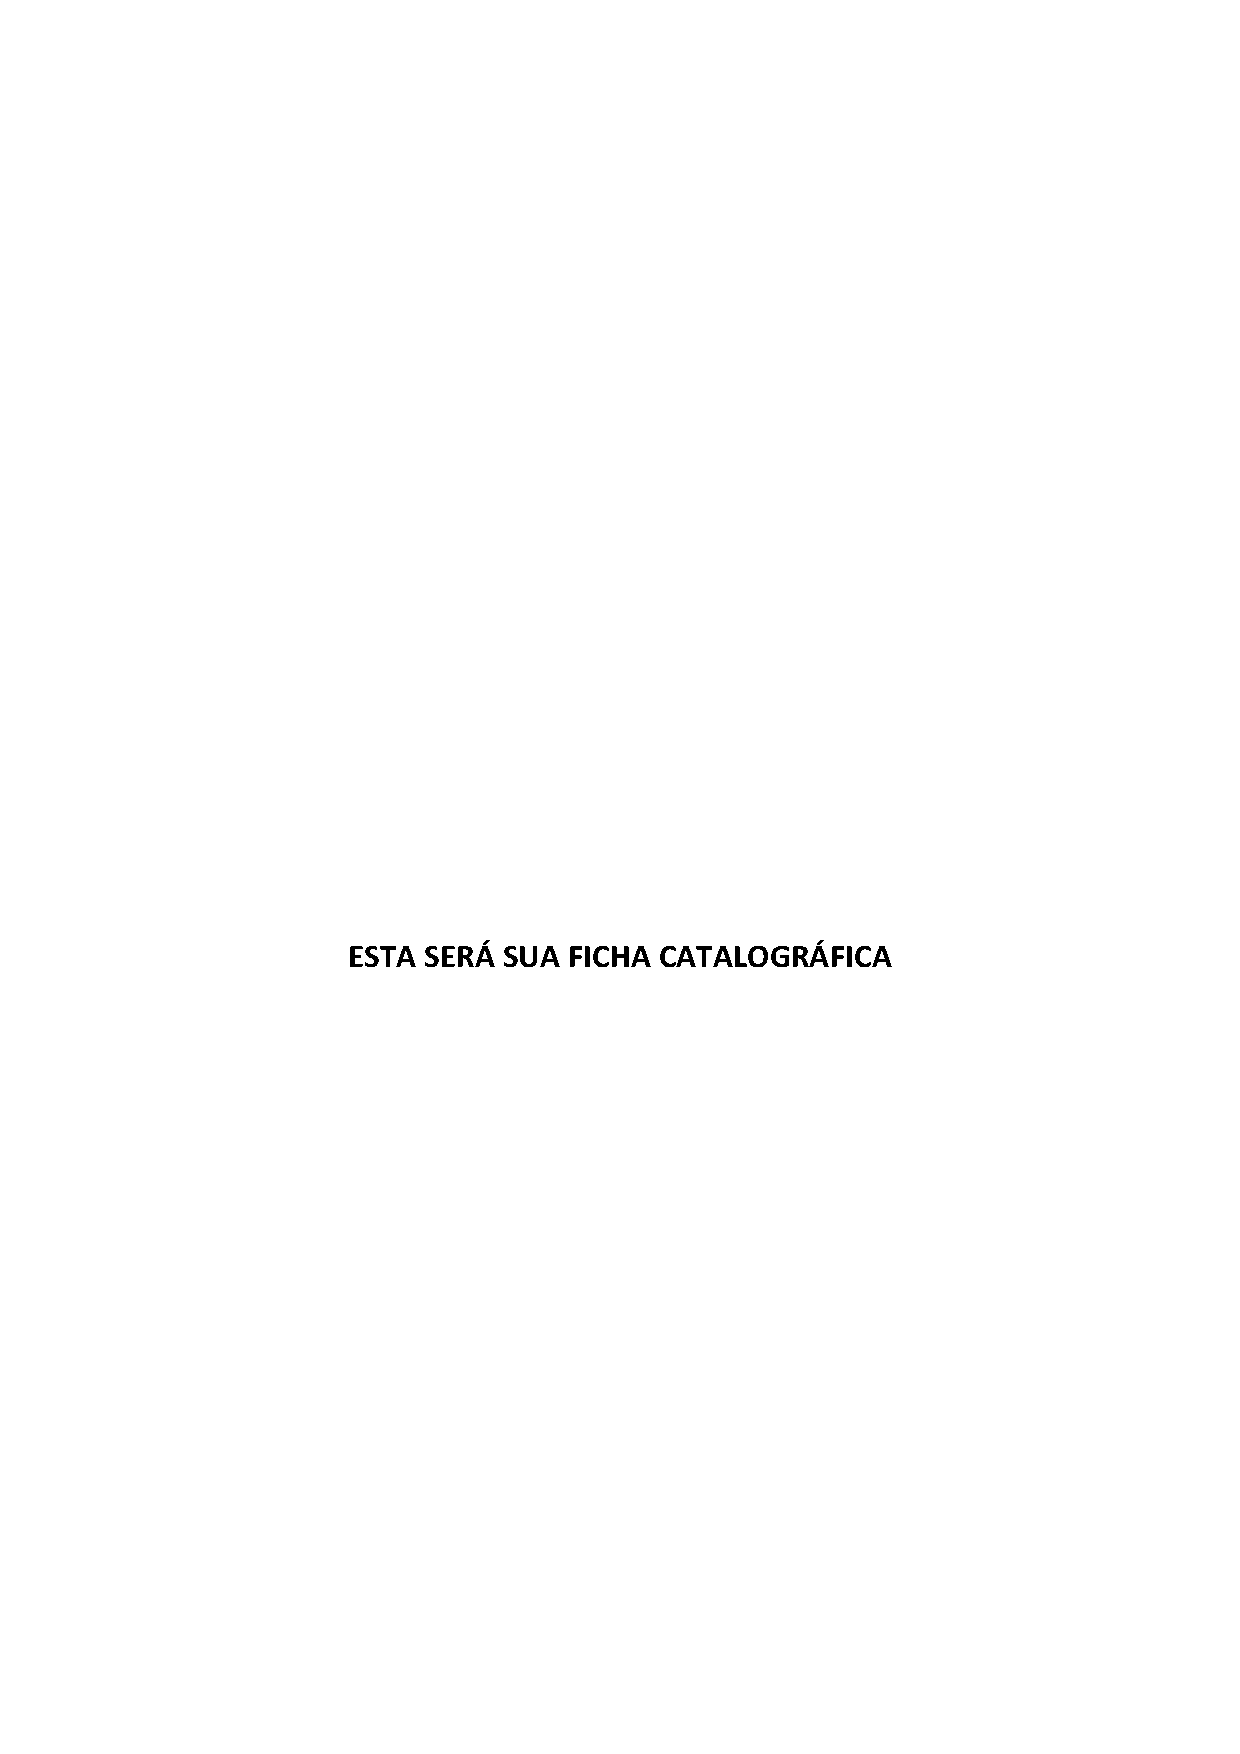
\includepdf[pages=-]{anexos/ficha.pdf}

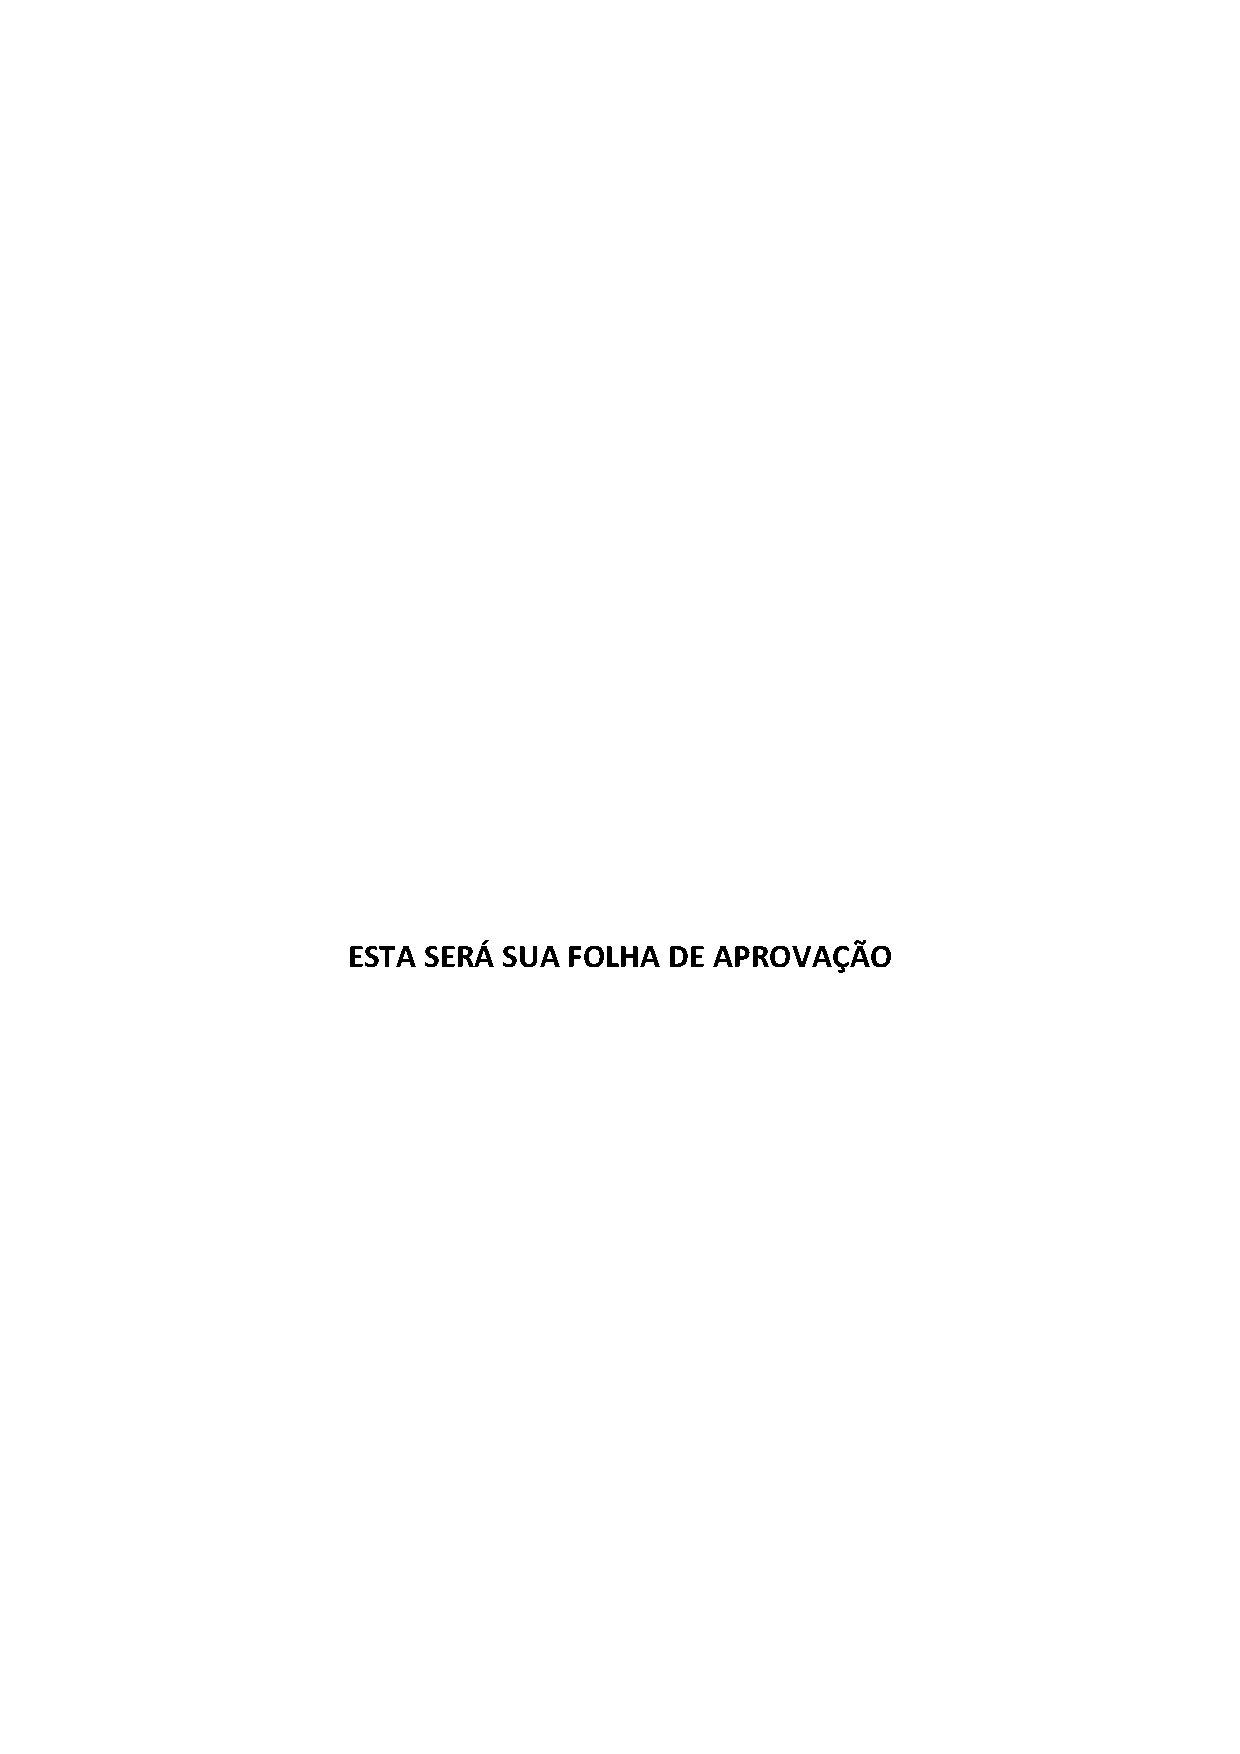
\includepdf[pages=-]{anexos/aprovacao.pdf}

\setlength{\ABNTEXsignwidth}{12cm}

%--------------------------------------------------------------------------------
% Está comentado pelo mesmo motivo da ficha catalográfica
%--------------------------------------------------------------------------------
%\begin{folhadeaprovacao}
%	\begin{center}
%	    {\ABNTEXchapterfont\bfseries\large\imprimirinstituicao}
%	    \vspace*{\fill}
%
%	    {\ABNTEXchapterfont\bfseries\large FOLHA DE APROVAÇÃO}
%	    \vspace*{\fill}
%
%	    {\ABNTEXchapterfont\bfseries\large\imprimirautor}
%
%	    \vspace*{\fill}\vspace*{\fill}
%	    {\ABNTEXchapterfont\bfseries\large\imprimirtitulo}
%	    \vspace*{\fill}
%
%	    {\hspace{.45\textwidth}
%		\begin{minipage}{.5\textwidth}
%			\SingleSpacing
%			\ABNTEXchapterfont\imprimirpreambulo \\ \\
%
%			{\ABNTEXchapterfont\imprimirorientadorRotulo~\imprimirorientador\par}
%			{\ABNTEXchapterfont\imprimircoorientadorRotulo~\imprimircoorientador\par}
%
%		\end{minipage}%
%	    \vspace*{\fill}}
%	\end{center}
%
%	\vspace*{\fill}
%
%	\begin{center}
%			 \ABNTEXchapterfont\large Aprovado em: \_\_\_\_ de \_\_\_\_ de 2017
%	\end{center}

%	\vspace*{\fill}

%	\begin{center}
%			 \ABNTEXchapterfont\bfseries\large Banca Examinadora
%	\end{center}
%
%   \ABNTEXchapterfont\assinatura{Fábio Nelson de Sousa Pereira, Mestre, Universidade Federal do Vale do São Francisco}
%	\ABNTEXchapterfont\assinatura{Jorge Luis Cavalcanti Ramos, Doutor, Universidade Federal do vale do São Francisco}
%  \ABNTEXchapterfont\assinatura{Ricardo Argenton Ramos, Doutor, Universidade Federal do Vale do São Francisco}
%	 \vspace*{\fill}


%\end{folhadeaprovacao}

%-------------------------------------------------------------------------------
% Insere a epígrafe
%-------------------------------------------------------------------------------
\newpage
\vspace*{\fill}
\begin{flushright}
    \textit{Lorem Ipsum...}
\end{flushright}

%-------------------------------------------------------------------------------
% Seção de agradecimentos
%-------------------------------------------------------------------------------
\begin{agradecimentos}

\lipsum[2-4]

\end{agradecimentos}

%-------------------------------------------------------------------------------
% Insere a segunda epígrafe
%-------------------------------------------------------------------------------
\begin{epigrafe}
  \vspace*{\fill}
  \begin{flushright}
    Se pude enxergar a tão grande distância, foi subindo nos ombros de gigantes.\\
     \vspace{\baselineskip}
    \textbf{Isaac Newton}\\
    \textbf{Carta à Robert Hooke, 1676}
  \end{flushright}
\end{epigrafe}



%-------------------------------------------------------------------------------
% Seção de resumos
%-------------------------------------------------------------------------------
% resumo em português
\setlength{\absparsep}{18pt} % ajusta o espaçamento dos parágrafos do resumo
\begin{resumo}

  Os avanços do acesso às tecnologias da informação criou um ambiente fértil
  para a pesquisa na área de ensino à distância. Porém, apesar da grande
  disponibilidade e flexibilidade, os cursos da modalidade EAD, no Brasil, ainda
  sofrem com o problema da evasão de estudantes, como vem sendo mostrado no
  Censo EAD.BR dos ultimos anos. Acompanhando o crescimento da EAD, se
  desenvolve também a área de Mineração de Dados Educacionais. Inspirado pela
  Teoria da Distância Transacional, este trabalho propõe a utilização da
  metodologia de descoberta de conhecimento em bancos de dados para construir e
  comparar modelos de classificação da situação final de um aluno de curso EAD
  entre duas classes, evasor ou não-evasor. Este trabalho aplica a metodologia
  proposta por Ramos et al (2016), onde as variáveis utilizadas nos modelos
  preditivos são construídas com base nos construtos da TDT, comparando os
  resultados obtidos com um novo cenário educacional.

  \textbf{Palavras-chave}: Educação à distância. Mineração de dados
  educacionais. Evasão escolar.

\end{resumo}
\newpage

% resumo em inglês
\begin{resumo}[Abstract]
\begin{otherlanguage*}{english}

  The advances in information technologies created a very fertile research
  environment in the distance education field. However, despite of the great
  disponibility and flexibility, the   brazilian DE course genre still suffers
  from the students evasion problem, as shown by the EAD.BR census in the last
  few years. Along with the growing in DE, the Educational Data Mining is
  developing as well. Inspired by the Transactional Distance Theory, this works
  proposes the using of knowledge discovery in databases to construct and
  compare classification models on the final situation of a DE student between
  two classes, evasor and not-evasor. This work applies the methodology proposed
  by Ramos et al (2016), where the variables utilized in the predictive models
  are constructed based on the TDT attributes, comparing the results found with
  a new educational scenario.

  \textbf{Key-words}: Distance education. Educational data mining. School
  evasion.

\end{otherlanguage*}
\end{resumo}


%-------------------------------------------------------------------------------
% Insere lista de ilustrações
%-------------------------------------------------------------------------------
\begin{KeepFromToc} % Este comando evita que todas as seções dentro dele de apareçam no sumário
\pdfbookmark[0]{\listfigurename}{lof}
\listoffigures
\cleardoublepage


%-------------------------------------------------------------------------------
% Insere lista de tabelas
%-------------------------------------------------------------------------------
% \pdfbookmark[0]{\listtablename}{lot}
% \listoftables
% \cleardoublepage

%-------------------------------------------------------------------------------
% Insere lista de quadros
%-------------------------------------------------------------------------------
% \pdfbookmark[0]{\listofquadrosname}{loq}
% \listofquadros*
% \cleardoublepage

%-------------------------------------------------------------------------------
% Ajusta lista de código - alterar de figures para códigos - by @Gabrielr2508
%-------------------------------------------------------------------------------
% \makeatletter
% \let\l@listing\l@figure
% \def\newfloat@listoflisting@hook{\let\figurename\listingname}
% \makeatother

%-------------------------------------------------------------------------------
% Insere lista de códigos - by @leolleocomp
%-------------------------------------------------------------------------------
% \listoflistings

\end{KeepFromToc}

%-------------------------------------------------------------------------------
% Insere lista de abreviaturas e siglas
%-------------------------------------------------------------------------------
% \begin{siglas}
%   \item[LI]       Lorem Ipsum
%   \item[LII]		Lorem Ipsum Ipsum

% \end{siglas}

%-------------------------------------------------------------------------------
% Insere o sumario
%-------------------------------------------------------------------------------
\pdfbookmark[0]{\contentsname}{toc}
\tableofcontents*
\cleardoublepage


